%------------------------------------------------------------------------------

\chapter{Υλοποίηση}
\label{chapter4}

\section{Γενικά}

Σε αυτό το κεφάλαιο θα αναλύσουμε τις λεπτομέρειες περί της υλοποίησης και τις
δυσκολίες που προέκυψαν σε αυτή. Η βάση μας είναι ένα προηγούμενο paper των
Standler, W{\"u}rthinger et al\cite{stadler2014partial} που μελετά, περιγράφει
και υλοποιεί την μέθοδο για την γλώσσα Java. Ακολουθήσαμε σε γενικές γραμμές –
και ειδικότερα στην αρχή – τις περιγραφές που δίνουν για την υλοποίηση και
δομήσαμε την υλοποίησή μας όμοιως. Βέβαια όσο προχωρούσαμε τόσο αποκλίναμε από
αυτή την περίπτωση, καθώς εμείς είχαμε να κάνουμε με μια δυναμική γλώσσα σε
αντίθεση με την στατική Java. Επιπλέον πολλές λεπτομέρειες έλειπαν από την
εργασία.

Ο κυρίως κώδικας (δηλαδή το αρχείο \texttt{partial\_escape.py}) δίνεται στο
παράρτημα Α'. Οι γραμμές κώδικα που εμφανίζονται στο παρακάτω κείμενο
αναφέρονται σε αυτόν.

Όπως έχουμε ήδη αναφέρει ο κώδικας του project του PyPy χωρίζεται σε
subsystems, και modules. Το module που υλοποιούμε υπόκειται στο σύστημα
RPython, στο subsystem του translator, στην ομάδα των backend
βελτιστοποιήσεων. Βρίσκεται επομένως στο ακόλουθο μονοπάτι:
\path{pypy/rpython/translator/backendopt/partial_}\\ \path{escape.py}. Ο κώδικας
βρίσκεται σε ένα fork\cite{fork} του επίσημου \textit{repository} του
PyPy\cite{repo} στη σελίδα bitbucket\footnote{\url{http://bitbucket.com}}. Η
υλοποίηση έγινε με την βοήθεια του εργαλείου διαχείρησης εκδόσεων κώδικα (SCM)
mercurial\cite{mercurial} το οποίο χρησιμοποιείται και εσωτερικά από το
project. Φυσικά γίνονται προσπάθειες προκειμένου το module μας να
συμπεριληφθεί στο επίσημο repo του PyPy.


\subsection*{Test-driven development}

Στην υλοποίηση χρησιμοποιήθηκε η μέθοδος ανάπτυξης λογισμικού βασισμένη σε
tests (\textit{test-driven development}\cite{tdd}). Είναι μια σχετικά
καινούργια μέθοδος ανάπτυξης που χρησιμοποιεί test κώδικα για να ελέγξει την
ορθότητα του κανονικού κώδικα των προγραμμάτων. Η μέθοδος αναπτύχθηκε φυσικά
λόγω της μεγάλης πολυπλοκότητας που έχουν τα διάφορα προγράμματα και συστήματα
την σήμερον ημέρα. Ο προγραμματιστής αφού κατανοήσει περίπου πως πρέπει να
δομήσει το πρόγραμμα του ξεκινά με την συγγραφή του test κώδικα. Αρχικά για
τις απλές (και ίσως τετριμένες) περιπτώσεις και σταδιακά αυξάνει την
πολυπλοκότητα των tests και φυσικά του κώδικα αντιστοίχως. Αφού γράψει ένα ή
περισσότερα tests, συγγράφει το πρόγραμμά του προσπαθώντας να κάνει τα tests
να ``τρέξουν" επιτυχώς. Η διαδικασία συνεχίζεται φυσικά μέχρι να ολοκληρωθεί η
διαδικασία ανάπτυξής ή να φτάσει ο προγραμματιστής στην επιθυμητή
πολυπλοκότητα. Με αυτόν τον τρόπο – αν προφανώς όλα τα tests είναι επιτυχή – ο
προγραμματιστής είναι σίγουρος ότι οι καινούργιες αλλαγες που επέφερε στο
project δεν επηρέασαν την ορθότητα του προγράμματος σε κάποιο προηγούμενο
στάδιο.

Το PyPy χρησιμοποιεί αυτή την μέθοδο, οπότε και η υλοποίησή μας την ακολουθεί.
Ο test κώδικας του module που υλοποιήθηκε βρίσκεται στο ακόλουθο μονοπάτι:
\path{pypy/rpython/translator/backendopt/test/test_partial_escape.py}. Δεν
συμπεριλαμβάνεται στην εργασία αυτή για λόγους λακωνικότητας.

%------------------------------------------------------------------------------

\section{Δομή του κώδικα}

\subsection{Βασική Συνάρτηση}

Ο κώδικας είναι σε ένα αρχείο. Χωρίζεται φυσικά σε συναρτήσεις. Η κυρίως
συνάρτηση είναι η \texttt{partial\_escape()}. Αυτή αποτελεί το κυρίως module που
θα τρέξει για κάθε γράφημα με σκοπό την βελτιστοποίηση. Το σύστημα θα καλεί την
συνάρτηση αυτή δίνοντας της ένα γράφημα την φορά σε ένα loop. Τα διαθέσιμα
γραφήματα θα είναι όλες οι συναρτήσεις του μεταγλωττιστή. Το γράφημα
μεταβάλλεται \textit{in-place} και το return value είναι ένας μετρητής των
\texttt{getfield} εντολών που αφαιρέθηκαν. Πρακτικά η μείωση των εντολών
\texttt{getfield} στο γράφημα είναι ο κύριος στόχος της συνάρτησης καθώς το
module μας θα τρέξει μετά το ήδη υπάρχον module για ανάλυση διαφυγής (non-
partial escape analysis) στο PyPy. Παρόλα αυτά δεν είναι μόνο αυτή η αλλαγή που
επιφέρεται από το module. Σίγουρα αφαιρούνται πολλές εντολές \texttt{malloc} –
οι οποίες είναι εξαιρετικά ακριβές. Επιπλέον πολλές ακριβές εντολές
μετακινούνται σε κάποιο μονοπάτι της ροής εκτέλεσης το οποίο εκτελείται σπάνια ή
λιγότερες φορές, οπότε εν δυνάμει είναι σαν να αφαιρούνται.


\subsection{worklist}

Με τον όρο \textit{Worklist} καλούμε την δομή δεδομένων που χρησιμοποιούμε για
να μας βοηθά στην επιλογή του επόμενου \texttt{Block} προς επεξεργασία.
Επιλέξαμε ένα deque\cite{deque} (από τα εσωτερικά structures της Python από το
module \texttt{collections}). Γενικά, στον κώδικα, χρησιμοποιούμε πολύ συχνά
constructions της Python προς διευκόλυνσή μας. Ένα deque ή dequeue
(\textit{double ended queue}) είναι μια ουρά (queue) που έχει δυνατότητα
εισαγωγής και εξαγωγής και από τις δύο άκρες. Η επιλογή του επόμενου
\texttt{Block} εξαρτάται από πολλούς παράγοντες – η μεγαλύτερη πολυπλοκότητα
απαντάται στην περίπτωση των loops, καθώς κάθε \texttt{Block} πρέπει να
επεξεργαστεί προφανώς μόνο μια φορά και στην σωστή σειρά. Μια τέτοια δομή
δεδομένων ήταν η ιδανική για τον σκοπό μας. Η επεξεργασία του \textit{worklist}
γίνεται στο τέλος κάθε iteration επεξεργασίας κάποιου \texttt{Block} (στις
γραμμές $371-381$ του κώδικα.)

\subsection{Αφαίρεση μεταβλητών και αντικατάσταση με βαθμωτούς}

Όταν ο μεταγλωττιστής εντοπίσει μια καινούργια μεταβλητή τότε την αφαιρεί από
τον κώδικα, δημιουργεί ένα εικονικό αντικείμενο (βλ. παρακάτω) και την
``παρακολουθεί". Δηλαδή ανιχνεύει τις ενέργειες που γίνονται με αυτή, καταγράφει
τις εντολές που τρέχουν και τις αντικαθιστά αναλόγως, έτσι ώστε η λογική, η
εκτέλεση, και η ορθότητα του προγράμματος να παραμένει ίδια παρόλο που
αφαιρέσαμε μια ολόκληρη μεταβλητή. Για παράδειγμα το παρακάτω κομμάτι κώδικα:

\begin{lstlisting}[language=Python, deletendkeywords={id}]
k = Key()
k.id = 1
\end{lstlisting}

θα μεταφραστεί σε:

\begin{lstlisting}[language=Python, deletendkeywords={id}, keywords={malloc}]
k1 = malloc(...)
setfield(k1, id, 1)
\end{lstlisting}

Εκτός από την αφαίρεση της εντολής \texttt{malloc} εδώ, θα αφαιρεθεί επίσης και
η εντολή \texttt{setfield}, καθώς έχει να κάνει με το αντικείμενο που
αφαιρείται. Εκτός από την αφαίρεση, η κάθε εντολή έχει φυσικά και συνέπειες για
τα εικονικά αντικείμενα. Για παράδειγμα η \texttt{setfield} προκαλεί το
\textit{set} σε ένα από τα fields του εικονικού αντικειμένου σύμφωνα με τα
ορίσματά της. Στο παραπάνω παράδειγμα θα δημιουργηθεί ένα field ``id" στο
εικονικό αντικείμενο. Επίσης (εκτός από την \texttt{malloc} και την
\texttt{setfield}) υπάρχουν και άλλες εντολές που είτε μεταβάλλονται είτε
μεταβάλλουν τα εικονικά αντικείμενα. Η σημαντικότερη από αυτές είναι η εντολή
\texttt{getfield}. Αυτή η εντολή είναι το σημείο που θα γίνει η πραγματική
αντικατάσταση βαθμωτού, καθώς εκεί είναι απαραίτητη η τιμή. Το \texttt{getfield}
κάνει το access σε κάποιο field μιας μεταβλητής. Εάν εμείς αφαιρέσουμε την
μεταβλητή θα πρέπει να αντικαταστήσουμε την τιμή εδώ με κάποιον αντίστοιχο
βαθμωτό ή με κάποιον υπολογισμό, σύμφωνα πάντα με τα συμφραζόμενα. Η
``πιστοποίηση" για το αν οι εντολές επηρεάζουν τα εικονικά αντικείμενα γίνεται
πολύ απλά με έναν έλεγχο για το αν το αντικείμενο υπάρχει μέσα στο
\textit{state}. Αν δεν υπάρχει τότε η εντολή έχει να κάνει με κάποιο αντικείμενο
που δεν μπορούμε να πειράξουμε είτε με κάποιο που έχει ήδη επανατοποθετηθεί (βλ.
επόμενη παράγραφο).

\subsection{materialization}

Με τον όρο \textit{materialization} καλούμε την ``επανατοποθέτηση" του
αντικειμένου στον κώδικα. Αυτό περιλαμβάνει την επανατοποθέτηση των εντολών για
την δέσμευση της μνήμης και οποιασδήποτε αρχικοποίησης ή τυχών casting ή
aliasing πρέπει να εφαρμοστεί στο αντικείμενο, καθώς και την ``ακύρωση"
οποιονδήποτε άλλων ενεργειών έχουμε ήδη εκτελέσει. Οι κυρίως λόγοι που μπορεί να
προκαλέσουν κάποιο αντικείμενο να κάνει materialization είναι η επιστροφή του ως
return value ή το globaliazation του, δηλαδή η αλλαγή scope του (η ανάθεσή του,
με άλλα λόγια, σε κάποια global μεταβλητή). Οι ενέργειες που πρέπει να γίνουν
φυσικά διαφέρουν ανάλογα με το αντικείμενο και ανάλογα με το πόσες εντολές (π.χ.
\texttt{setfield}) έχουν εκτελεστεί σε αυτό. Οι εντολές για την αρχικοποίησή του
(\texttt{malloc} και \texttt{cast}) θα τοποθετηθούν είτε στο προηγούμενο Block
είτε στο τρέχον. Στο τρέχον θα τοποθετηθούν αν ο μεταγλωττιστής ανακαλύψει την
ανάγκη για materialization πάνω στην κανονική επεξεργασία των εντολών ενώ στο
προηγούμενο αν την ανακαλύψει οπουδήποτε αλλού (π.χ. κατά την επεξεργασία των
link arguments).

Η πιο περίπλοκη περίπτωση είναι αυτή που το αντικείμενο περιέχει ένα reference
σε άλλο εικονικό αντικείμενο. Αν ένα εικονικό αντικείμενο πρέπει να υλοποιηθεί
ξανά (materialization) τότε πρέπει να συμβεί το ίδιο και για όλα τα εικονικά που
περιέχει. Αυτό το διαχειριζόμαστε με recursion στην συνάρτηση του
materialization, οπότε ακολουθούνται οι ίδιες ενέργειες.

Υπάρχει επίσης μια bypass δυαδική μεταβλητή η οποία μπορεί να εξαναγκάσει το
materialization (\texttt{must\_be\_materialized}).


\subsection{aliasing}

Η Python είναι δυναμική οπότε τα εσωτερικά castings των μεταβλητών και τα
διαφορετικά ονόματά τους (\textit{aliases}) βρίθουν. Το σύστημά μας έπρεπε να
διαχειρίζεται τα castings και να ακολουθεί το σύστημα με τα aliasings που
περιγράφεται από το paper έτσι ώστε να καλύψει τις περιπτώσεις όλων των
ονομάτων για τις ίδιες μεταβλητές – Η Python πολλές φορές χρησιμοποιεί
διαφορετικά ονόματα για την ίδια μεταβλητή προκειμένου να χρησιμοποιήσει
λιγότερη μνήμη. Το paper κηρύττει την χρήση ενός δεύτερου dictionary που θα
``δείχνει" στο \textit{id} που με την σειρά του θα ``δείχνει" στο εικονικό
αντικείμενο. Εμείς – αφού έχουμε στην διάθεσή μας τις κατασκευές και ευκολίες
που προσφέρει η Python – χρησιμοποιούμε επιπλέον keys (στο ίδιο dictionary)
που απλά ``δείχνουν" στο ίδιο εικονικό αντικείμενο. Με αυτόν τον τρόπο
διατηρούμε κάθε όνομα που υπάρχει για την μεταβλητή και μπορούμε να
``ανιχνεύουμε" για αυτά τον κώδικα κατά την μεταγλώττιση. Εκτός από αυτό,
διατηρούμε και ένα \textit{set} από τα ίδια κλειδιά/ονόματα μέσα σε κάθε
εικονικό αντικείμενο έτσι ώστε να ξέρουμε εύκολα τα κλειδιά όταν πρέπει να
επανατοποθετήσουμε το αντικείμενο στον κώδικα (βλ. materialization), αφού
προφανώς πρέπει να ``υπακούει" και πάλι σε όλα τα ονόματα που είχε. Το
\textit{set} αυτό αρχικοποιείται, φυσικά, στην \texttt{\_\_init\_\_()}
συνάρτηση του \texttt{VirtualObject}.

\subsection{Άλλες συναρτήσεις και κλάσεις}

\subsubsection{VirtualObject}

Η κυρίως κλάση του module. Αντιπροσωπεύει ένα εικονικό αντικείμενο και περιέχει
ότι χρειάζεται. Είναι σχετικά απλή καθώς οι περισσότερες διαδικασίες διαχείρησης
λαμβάνουν χώρα στις συναρτήσεις. Περιέχει μόνο μια μέθοδο λ.χ. η οποία είναι η
\texttt{indencical\_malloc\_args()} και αυτό που κάνει είναι απλά να ελέγχει αν το
εκάστοτε στιγμιότυπο στο οποίο τρέχει (\textit{self}) και ένα όρισμά της, έχουν
ίδια ορίσματα στην εντολή δέσμευσης μνήμης. Η εντολή δέσμευσης μνήμης για το
κάθε αντικείμενο αποθηκεύεται μέσα στο αντίστοιχο εικονικό αντικείμενο πριν το
πρώτο αφαιρεθεί από τον κώδικα. Έκτος από αυτό, κάθε τέτοιο εικονικό αντικείμενο
αποθηκεύει ένα dictionary με όλα τα πεδία (\textit{fields}) – που μπορεί να
περιείχε το αρχικό αντικείμενο, τον τύπο του cast για το malloc του
αντικειμένου και ένα σετ με όλα τα aliases (βλ. [που?]) για το αντικείμενο.

\subsubsection{get\_current\_state()}

Απλή, βοηθητική συνάρτηση η οποία δέχεται ως όρισμα μια λίστα η οποία περιέχει
dual tuples - ζευγάρια δηλαδή, από \texttt{Link}s και \textit{states}. Αποτελεί
μια wrapper συνάρτηση που κάνει μικρότερης σημασίας τετριμμένες εργασίες. Στις
περισσότερες φορές το μέγεθος της λίστας είναι 1 (σειριακή περίπτωση) και
επιστρέφεται αμέσως το \textit{state}. Σε άλλες καλείται η συνάρτηση
\texttt{merge()} Δέχεται επίσης την bypass μεταβλητή
\texttt{must\_be\_materialized} και την περνάει στις επόμενες συναρτήσεις όπου
χρειάζεται.

\subsubsection{can\_remove()}

Απλή, βοηθητική συνάρτηση η οποία χρησιμοποιείται για να κρίνει εάν το δοθέν
αντικείμενο μπορεί να αφαιρεθεί με ασφάλεια. Οι έλεγχοι που κάνει είναι
δευτερεύοντες, καθώς το αν το αντικείμενο μπορεί να αφαιρεθεί ή όχι είναι το όλο
νόημα της βελτιστοιποίησης αυτής. Περιλαμβάνουν τελικούς ελέγχους για το αν το
αντικείμενο λ.χ. έχει destructors\footnote{Εξαιρέσαμε τα αντικείμενα με
destructors από την ανάλυση γιατί αυξάνονταν η πολυπλοκότητα χωρίς πολύ κέρδος
στον χρόνο και στην μνήμη.} ή αν είναι υπόκειται σε garbage collection.

\subsubsection{remove\_virtual\_inputargs()}

Επίσης απλή, βοηθητική συνάρτηση που εκτελεί ένα είδους ``syncing" μεταξύ δύο
λιστών. Κάνει ένα iteration στα αντικείμενα του \textit{state} και διαγράφει την
αντίστοιχη μεταβλητή στα \texttt{inputargs} των \texttt{Block}s και των
\texttt{Link}s για οποιαδήποτε από αυτά υπάρχει. Αυτές είναι πλέον άχρηστες
καθώς χρησιμοποιούνταν πριν για να αναφερθούν σε αυτό, ενώ τώρα το αντικείμενο
δεν υπάρχει αφού είναι εικονικό.

\subsubsection{materialize\_object()}

Μια από τις τρεις δευτέροντες βασικές συναρτήσεις του module. Αναλαμβάνει το
materialization του αντικειμένου για το οποίο θα καλεστεί. Δέχεται ως όρισμα το
``κλειδί" του αντικειμένου αυτού στο \textit{state}, το ίδιο το \textit{state}
και την λίστα με τις εντολές (operations). Στην λίστα αυτή θα προστεθούν οι
εντολές που απαιτούνται. Αυτή μεταβάλλεται \textit{in- place} και
χρησιμοποιείται από την καλούσα συνάρτηση για να αντικαταστήσει τις εντολές του
\texttt{Block}.

Λειτουργεί επίσης ως ``κριτής" για την συνάρτηση που την κάλεσε, καθώς
επιστρέφει \texttt{True} ή \texttt{False} ανάλογα με το αν η λειτουργία της ήταν
επιτυχής.

\subsubsection{merge()}

Αυτή η συνάρτηση αναλαμβάνει να συγχωνεύσει δύο ή περισσότερα \textit{states} σε
ένα ανάλογα με τα εικονικά αντικείμενα και φυσικά το context από τα
\texttt{Block}s και τα \texttt{Link}s. Δέχεται (και αυτή) την λίστα με τα
δυαδικά tuples από \textit{states} και \texttt{Link}s. Καλείται μόνο από την
συνάρτηση \texttt{get\_current\_state()} εάν χρειάζεται, δηλαδή σε περιπτώσεις
if και loop. Η μεταβλητή \texttt{must\_be\_materialized} κυρίως επηρεάζει την
λειτουργία αυτής της συνάρτησης.

Για περισσότερες λεπτομέρειες βλ. παράγραφος Merge.

\subsubsection{copy\_state()}

Η τελευταία από τις τρεις δευτέροντες βασικές συναρτήσεις του module. Η
λειτουργία της είναι η αντιγραφή του \textit{state} για το επόμενο
\texttt{Block}. Φυσικά θα εκτελέσει και οποιεσδήποτε άλλες ενέργειες
απαιτούνται. Δέχεται προφανώς μια αντικείμενο \textit{state}, και επιπλέον ένα
\texttt{Link}\footnote{κυρίως απαιτούνται τα arguments και το target
\texttt{Block}}, και την ειδική μεταβλητή \texttt{must\_be\_materialized}.
Επιστρέφει ένα καινούργιο αντικείμενο \textit{state} φτιαγμένο για το καινούργιο
\texttt{Block}. Μπορεί με την πρώτη ματιά η υλοποίησή αυτής της συνάρτησης να
φαίνεται τετριμμένη, όμως έκρυβε δυσκολίες. Κατ' αρχάς η αντιγραφή ενός τέτοιο
dictionary είναι αυτή καθ' αυτή δύσκολη καθώς τα εικονικά αντικείμενα θα έχουν
διαφορετικά ονόματα στο επόμενο \texttt{Block} – δηλαδή άλλες μεταβλητές που θα
δείχνουν σε αυτά, οπότε πρέπει να αντιστοιχηθούν σωστά. Αυτό συμβαίνει γιατί το
σύστημα των γραφημάτων στο PyPy είναι προγραμματισμένο να χρησιμοποιεί
καινούργιες μεταβλητές σε κάθε καινούργιο \texttt{Block} για λόγους ανεξαρτησίας
των \texttt{Block}s. Η αντιστοιχία γίνεται ένα προς ένα μεταξύ των λιστών ενός
\texttt{Block} και ενός \texttt{Link}. Λ.χ. το πρώτο μέλος της λίστας από τα
arguments του \texttt{Block} θα μπει στην μεταβλητή που υπάρχει επίσης στο πρώτο
μέλος της λίστας του \texttt{Link}. Φυσικά αυτές οι λίστες θα πρέπει επίσης να
είναι ``συγχρονισμένες" με το ποια αντικείμενα είναι εικονικά και αυτές οι
αλλαγές λαμβάνουν χώρα εδώ. Όταν ένα αντικείμενο υπάρχει στο \textit{state} τότε
οποιαδήποτε μεταβλητή αναφέρεται σε αυτό στα arguments θα πρέπει να σβηστεί. Ο
κύριως σχεδιασμός της έγινε κατά την φάση υλοποίησης Split (βλ. παρακάτω).

%------------------------------------------------------------------------------

\section{Γραφήματα}

Η όλη διαδικασία ουσιαστικά αλλάζει το γράφημα που δέχεται ως είσοδο. Αν η
συνάρτησή μας δεχτεί ως όρισμα το γράφημα \ref{figure-2} τότε θα επιστρέψει το
βελτιστοποιημένο ως προς τα \texttt{mallocs} γράφημα που φαίνεται παρακάτω στο
\ref{figure-3}.

\begin{figure}[h]
\centering
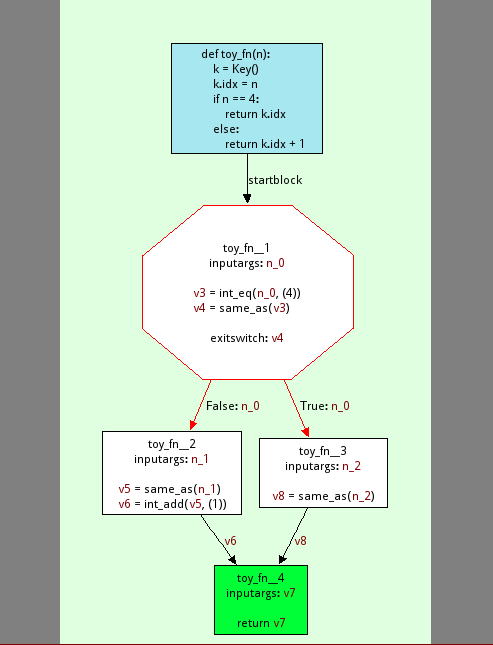
\includegraphics[width=0.6\textwidth]{simple-func-after.png}
\caption{Simple function flow diagram after the optimization took place.}
\label{figure-3}
\end{figure}

Φυσικά τα γραφήματα ακολουθούν τις τυπικές νόρμες που ακολουθούν όλα τα
μοντέλα γραφημάτων όπως \textit{SSA} και το απλό διάγραμμα ροής. Πολλές
\textit {προσωρινές-βοηθητικές} μεταβλητές που πρέπει να υπάρχουν στον κώδικα
αφαιρούνται γιατί ουσιαστικά μεταβάλλονται σε ``κατασκευές" στα γραφήματα κατά
το contruction – όπως π.χ. merge \texttt{Block}s. Στα γραφήματα, οι εξαρτήσεις
της ροής εκτέλεσης αναπαριστωνται ως έντονα βελάκια που δείχνουν προς τα κάτω
όπως επίσης φάινεται στο \ref{figure-3}.

\subsection{Πως μεταβάλλουμε τα γραφήματα}

Τα γραφήματα εσωτερικά ορίζονται στο \path{pypy/rpython/flowspace/model.py} και
σχεδιάζονται από το εξωτερικό module pygame. Μπορούμε μέσω μιας μεταβλητής graph
να βρούμε σειριακά όλα τα \texttt{Block} και \texttt{Link}s και μετά στο μέλος
\texttt{operations} του \texttt{Block} υπάρχει η λίστα με τις εντολές.
Μεταβάλλοντάς την μπορούμε να μεταβάλουμε το \texttt{Block} οπότε και το
γράφημα. Φυσικά τα παραπάνω είναι υπεραπλουστευμένα, αλλά δίνουν μια καλή
εικόνα. Για σωστή διαχείριση απαιτούνται επιπλέον πληροφορίες αλλά το σύστημα
του framework του PyPy παρέχει ότι μπορεί να χρειαστεί ο προγραμματιστής. Το
\texttt{Block} λ.χ. περιέχει επίσης λίστες με τα \textit{exits} του, λίστα με τα
ορίσματα που δέχεται\footnote{Το κάθε \texttt{Block} δέχεται – όπως και οι
συναρτήσεις – ορίσματα και ``επιστρέφει" μεταβλητές στα επόμενα μέσω των
\texttt{Link}s}, βοηθητικές συναρτήσεις (π.χ. \texttt{is\_final\_block()}), τη
μεταβλητή exitswitch που χρησιμοποιείται για τα branches (ifs), και τέλος
πληροφορίες για την διαχείριση του από το σύστημα του μεταγλωττιστή και από το
σύστημα που τα ``ζωγραφίζει" στην οθόνη. Τα \texttt{Link}s περιέχουν τα
αντίστοιχα arguments και την μεταβλητή \texttt{target} που ``δείχνει" στο επόμενο
\texttt{Block}. Επιπλέον περιέχουν τις ειδικές μεταβλητές
\texttt{last\_exception} \& \texttt{last\_exc\_value} που χρησιμοποιεί το
μοντέλο για την διαχείριση των εξαιρέσεων και φυσικά όπως και τα
\texttt{Block}s, εσωτερικές πληροφορίες. Από τα περιεχόμενα των graph μεταβλητών
αυτά που πρέπει να τονίσουμε είναι τα \texttt{exceptblock} \texttt{returnblock}
\texttt{startblock}. Τέλος περιέχει τους iterators που χρησιμοποιούμε για να
αποκτήσουμε τα \texttt{Block}s.

Να αναφέρουμε επίσης ότι το framework περιλαμβάνει πολλές χρήσιμες συναρτήσεις
και κατασκευάσματα που βοηθούν σε μεγάλο βαθμό το έργο του προγραμματιστή. Ακόμα
και σε τόσο χαμηλό επίπεδο προγραμματισμού οι βοηθητικές αυτές συναρτήσεις είναι
πάντα καλοδεχούμενες και βοηθούν στην ταχύτατη ανάπτυξη. Μερικές από αυτές
παραθέτονται παρακάτω. Τις περισσότερες φορές το όνομα τους αρκεί για την
κατανόηση. Σε αντίθετη περίπτωση τις εξηγούμε συνοπτικά.

\begin{itemize}

\item \texttt{mkentrymap()} Δέχεται ένα γράφημα και επιστρέφει ένα λεξικό
(\textit{dictionary}). Τα κλειδιά (keys) είναι τα \texttt{Block}s και τα values
είναι λίστες με όλα τα \texttt{Links} που δείχνουν στο εκάστοτε \texttt{Block}
του κλειδιού

\item \texttt{find\_backedges()} Όμοιως δέχεται ένα γράφημα και επιστρέφει μια
λίστα Python με όλες τις ακμές επιστροφής (\textit{backedges}) του γραφήματος.
Ένα back edge σε ένα γράφημα είναι μια ακμή η οποία δείχνει σε έναν προηγούμενο
κόμβο ο οποίος έχει ήδη καταγραφεί από τις κανονικές ακμές του
δέντρου/γραφήματος.

\item \texttt{find\_loop\_blocks()}

\end{itemize}

Μετά το πέρας της δικιά μας βελτιστοποίησης τρέχουμε επίσης κάποιες συναρτήσεις
``καθαρισμού" των \texttt{Block}s έτσι ώστε να αφαιρέσουν τυχόν απομεινάρια
εντολών ή εντολές που πλέον δεν απαιτούνται. Για παράδειγμα πολλές φορές μένουν
στον κώδικα εντολές \texttt{same\_as} (μετονομάσιας μεταβλητών) για μεταβλητές
που αφαιρέσαμε κατά την βελτιστοποίηση. Αυτές είναι:

\begin{itemize}

\item \texttt{remove\_same\_as()} Αφαιρεί τα \texttt{same\_as}

\item \texttt{transform\_dead\_op\_vars()} Αφαιρεί μεταβλητές που ορίζονται αλλά
δεν χρησιμοποιούνται.

\end{itemize}

%------------------------------------------------------------------------------

\section{Φάσεις σχεδιασμού}

Εδώ θα αναλύσουμε τον τρόπο σκεψης που ακολουθήσαμε για τον σχεδιασμό του module
αυτού. Ξεκινήσαμε προφανώς από την απλούστερη περίπτωση και ακολουθώντας φυσικά
τον προγραμματισμό με βάση τα tests. Ανεβαίνουμε σε πολυπλοκότητα άπαξ και τα
tests είναι επιτυχή, προσθέτοντας κάθε φορά και ένα κομμάτι.

\subsection{Σειριακά}

Αρχικά ξεκινάμε με την περίπτωση που ολόκληρο το σώμα του κώδικα βρίσκεται σε
ένα μόνο \texttt{Block} και δεν υπάρχει καμία πολυπλοκότητα στην ροή του
γραφήματος όπως loops ή if branches. Εδώ στοχεύουμε στο να κατασκευάσουμε την
αρχική μορφή και βασική λειτουργία του module μας. Όσο έχει να κάνει δηλαδή με
την λειτουργία στην ``παρακολούθηση" των μεταβλητών μέσα στα \texttt{Block}s.
Αφού τα \texttt{Block}s είναι το κυρίως κομμάτι των γραφημάτων, η ανάλυση μέσα
σε αυτά είναι από τα πιο σημαντικά κομμάτια του εγχειρήματός μας. Παρακάτω (στην
εικόνα \ref{figure-4}) δίνουμε πως εμφανίζεται ένα τέτοιο απλό γράφημα. Τα tests
περιλάμβαναν περιπτώσεις που κάποιο αντικείμενο έπρεπε να ``διαφύγει" – οπότε
ουσιαστικά το γράφημα παρέμενε απαράλλακτο, και περιπτώσεις που δεν έπρεπε οπότε
αφαιρούνταν.

\begin{figure}[h]
\centering
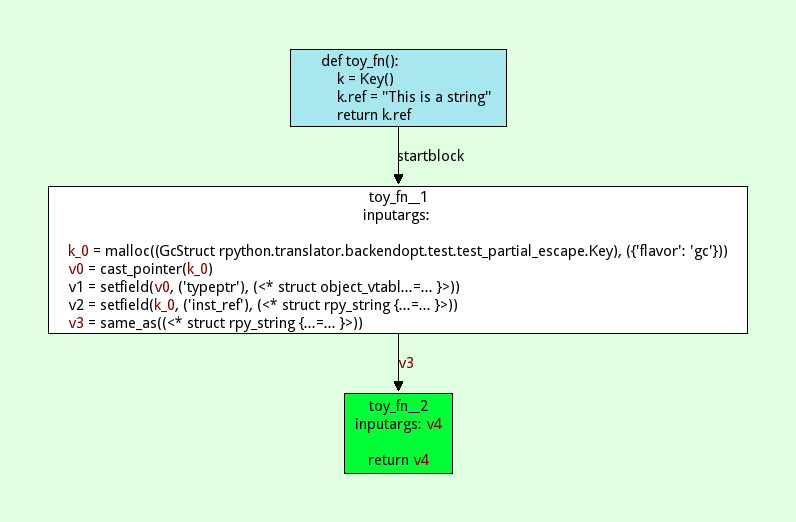
\includegraphics[width=0.8\textwidth]{simplest-func.png}
\caption{Very simple diagram. Screenshot from the diagram editor.}
\label{figure-4}
\end{figure}

Σε αυτού του είδους τα γραφήματα δημιουργείται μόνο ένα \textit{state}. Το
\textit{state} είναι η δομή δεδομένων την οποία χρησιμοποιούμε για να
αποθηκεύουμε την κατάσταση των μεταβλητών (όπως λέει και το όνομα) σε κάθε
\texttt{Block}. Περιέχει δηλαδή τα εικονικά αντικείμενα που αναπαριστούν
μεταβλητές. Εάν μια μεταβλητή αναπαριστάται στο \textit{state} αυτό σημαίνει ότι
μέχρι τώρα δεν διαφεύγει και έχει αφαιρεθεί από τον κώδικα. Ένα το σύστημα
αντιληφθεί ότι διαφεύγει τότε την επανατοποθετεί στον κώδικα  (όπως αυτό
χρειάζεται βλ. malloc και casts) και την αφαιρεί από το \textit{state}.

Αφού βελτιστοποιήσουμε τις εντολές μέσα στο μοναδικό \texttt{Block}, συνεχίζουμε
με τις επιπλέον περιπτώσεις. Να σημειώσουμε ότι πιο πριν ξεκινήσαμε χωρίς να
πειράξουμε το \texttt{Block} καθόλου έτσι ώστε να δούμε αν το σύστημα αλλάζει
λόγω side-effects. Φυσικά δεν υπήρχαν.

\subsection{Split}

\begin{wrapfigure}{H}{6.5cm}
\caption{State split. Screenshot from the diagram editor.}
\label{wrapped-figure}
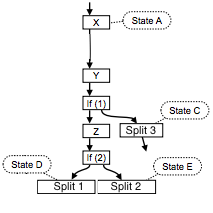
\includegraphics[width=6.5cm]{split-state.png}
\end{wrapfigure} 

Εδώ, στις συναρτήσεις (στις οποίες χρησιμοποιούνταν ως tests) είχαμε προσθέσει
ένα \textit{if}. Αυτό σημαίνει ότι η ροή θα μπορεί να ακολουθήσει δύο μονοπάτια
οπότε θα υπάρχουν παραπάνω από τρία \texttt{Block}s. Εμείς εδώ θα πρέπει να
προβλέψουμε το τι συμβαίνει σε όλα τα παρακλάδια της ροής εκτέλεσης.
Δημιουργούμε για αυτόν τον λόγο ένα \textit{state} για κάθε \texttt{Block}. Αν
έχουμε ένα \textit{split}, τότε το \textit{state} του αρχικού \texttt{Block} θα
αντιγραφεί στα άλλα \texttt{Block}s, και προφανώς το καθένα από αυτά θα
ακολουθήσει άλλη πορεία ζωής όταν γίνει η ανάλυση των επόμενων \texttt{Block}.
(Βλ. σχήμα \ref{wrapped-figure} δίπλα.)

Φυσικά αν υπάρχει \textit{split} από κάποιο \texttt{Block} με \textit{if}, τότε
θα υπάρχει και \textit{merge} σε κάποιο \texttt{Block} καθώς το
\textit{returnblock} κάθε γραφήματος είναι μοναδικό. Βέβαια όταν αυτό λαμβάνει
χώρα στο \textit{returnblock} δεν μας ενδιαφέρει καθώς το return γίνεται
αυτόματα και δεν πρέπει να αλλάξουμε κάτι, οπότε την διαχείριση των
\textit{merges} την έχουμε στο επόμενο επίπεδο δυσκολίας.

\subsection{Merge}

Σε αυτό το επίπεδο πολυπλοκότητας, δημιουργήσαμε tests και χειριστήκαμε τις
περιπτώσεις όπου τα \textit{merges} απαντώνται σε άλλα \texttt{Blocks} πλην
του \textit{returnblock}. Έπρεπε να διαχειριστούμε την ένωση δύο
\textit{state} μεταβλητών σε ένα. Εδώ ήταν το δυσκολότερο κομμάτι της
υλοποίησης καθώς οι λεπτομέρειες βρίθουν. Έπρεπε να ελέγξουμε και να
συγκρίνουμε τα δύο \textit{states}. Σε περίπτωση που ένα αντικείμενο υπήρχε
και στα δύο, τότε φυσικά έπρεπε να αντιγραφεί στο καινούργιο συγχωνευμένο και
να μεταφερθούν όλα τα περιεχόμενά του. Αυτή είναι η περίπτωση που το
αντικείμενο δεν έχει επηρεαστεί από το if branch (είτε δεν λάμβανε μέρος σε
αυτό) και μπορεί ακόμα να είναι εικονικό. Επίσης για να συμβεί το παραπάνω
πρέπει τα ορίσματα της εντολής δέσμευσης του αντικειμένου να είναι ίδια δηλαδή
το αντικείμενο να είναι πανομοιότυπο. Σε άλλες περιπτώσεις, δηλαδή όταν το
αντικείμενο είναι σε ένα από τα δύο \textit{states} dictionaries (είναι
εικονικό σε ένα μόνο branch), τότε το κάνουμε materialization και στα 2
branches, καθώς ο μεταγλωττιστής δεν μπορεί να ξέρει φυσικά σε ποιο θα
καταλήξει η ροή εκτέλεσης.

Σαφώς το \textit{merge} δεν λαμβάνει χώρα μόνο σε αυτές τις περιπτώσεις που
ξεκίνησαν με if αλλά και μετά από loops.

Να σημειώσουμε επίσης ότι η έκδοση της συνάρτησης που υλοποιεί το \textit{merge}
που παραθέτεται σε αυτή την εργασία είναι πολύπλοκη καθώς συμπεριλαμβάνει όλες
τις παραπάνω περιπτώσεις καθώς και τις περιπτώσεις των loops και του multi-merge
(βλ. επόμενη παράγραφος). Για μια πιο απλή κατανοητή έκδοση ανατρέχουμε στο log
του mercurial.

\subsection{Multi-merge}

Τα \textit{splits} είναι πάντα δυαδικά. Δηλαδή χωρίζονται σε δύο μόνο. Αν
υπάρχει τριπλό if case τότε το ένα από τα \texttt{Blocks} ξαναχωρίζεται. Τα
\textit{merges} όμως μπορούν να λάβουν χώρα όχι μόνο για δύο αλλά και για τρία
και παραπάνω \textit{Block}s σε ένα. Τότε η λογική για την συγχώνευση των
αντικειμένων \textit{state} θα πρέπει να τα λαμβάνει υπόψιν της.
Χρησιμοποιούμε ένα ζευγάρι για τον αρχικό έλεγχο – το οποίο είναι το αρχικό,
μοναδικό ζευγάρι στην περίπτωση απλής συγχώνευσης – και έπειτα εάν αυτός είναι
επιτυχής συγκρίνουμε με όσα αντικείμενα απομένουν. Η σύγκριση των ορισμάτων
για τον έλεγχο της ομοιότητας λαμβάνει χώρα στην – ορισμένη μέσα στο
αντικείμενο \texttt{VirtualObject} – μέθοδο \texttt{identical\_malloc\_args()}.

\subsection{Loops}

Η λογική των βρόγχων (loops) ήταν η δυσκολότερη. Μέχρι τώρα δεν έχουμε λάβει
υπόψιν μας τα loops στην λογική του προγράμματος. Όταν ο μεταγλωττιστής
εντοπίσει μια μεταβλητή που παίρνει μέρος σε ένα loop τότε την εξαναγκάζει να
διαφύγει. Ένα μεγάλο κομμάτι της σχεδίασης παρόλα αυτά (ακόμα και χωρίς την
κεντρική λογική) έχει υλοποιηθεί, και αυτό είναι το κομμάτι της διαχείρισης της
σειράς με την οποία \textit{βλέπουμε} και \textit{επεξεργαζόμαστε} τα
\texttt{Block}s (βλ. \textbf{worklist}). Στα μελλοντικά μας σχέδια
περιλαμβάνεται η πλήρης υλοποίηση της λογικής των loops. Παράδειγμα του πως
φαίνεται και υλοποιείται ένα γράφημα με loops δίνεται στο σχήμα \ref{figure-5}.

\begin{figure}[h]
\centering
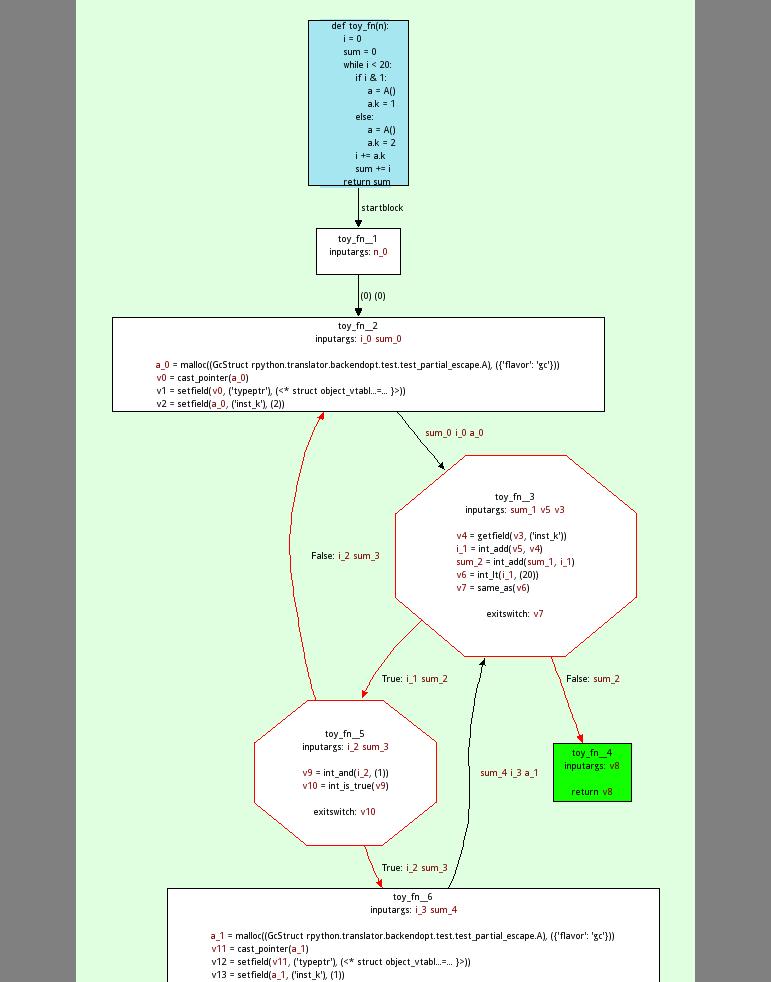
\includegraphics[width=0.7\textwidth]{loop-func.png}
\caption{Loop diagram. Screenshot from the diagram editor.}
\label{figure-5}
\end{figure}

\subsection{Function Calling etc}

Τέλος υπάρχουν επιπλέον επίπεδα πολυπλοκότητας που το σύστημα μπορεί να τα
διαχειριστεί μόνο του ή πολύ απλά η διαχείρισή τους να είναι τετριμμένη. Λ.χ. η
κλήση άλλων συναρτήσεων με την εντολή \texttt{direct\_call()} μπορεί απλά να
μείνει αυτούσια και να μην επηρεάζει την λογική μας. Φυσικά λαμβάνουμε υπόψιν τα
ορίσματα που παίρνει και επιστρέφει, καθώς αυτά μπορούν προφανώς να την
επηρεάσουν λ.χ. με την χρήση ενός αντικειμένου ως όρισμα.

%------------------------------------------------------------------------------

\section{Γενικά για προβλήματα}

Αρχικά να σημειώσουμε ότι δεν αντιμετωπίσαμε πολλά από τα προβλήματα που
αναφέρονταν στο paper\cite{stadler2014partial} που βασιζόμαστε, με βασικότερο
όλων την έλλειψη μηχανισμών κλειδώματος (locking). Αυτό το αποφύγαμε λόγω του
καθολικού κλειδώματος που υπάρχει στην Python και στην πλειοψηφία των
υλοποιήσεών της (Global Interpreter Lock – GIL). Το πρόβλημα με αυτή την
περίπτωση έγκειτο στο να συνειδητοποιήσουμε ότι δεν απαιτούνται επιπλέον
ενέργειες για την κάλυψη του locking.\cite{gil} Τα περισσότερα προβλήματα που
αντιμετωπίσαμε είχαν να κάνουν κυριώς με περιπτώσεις τις οποίες δεν είχαμε
σκεφτεί και δεν είχαμε προβλέψει.

\subsection{Edge cases}

Όπως είπαμε, σε ένα τέτοιο εγχείρημα, ακόμα και με την καλύτερη ανάλυση και τον
καλύτερο σχεδιασμό, θα προκύψουν θέματα που ο προγραμματιστής δεν είχε σκεφτεί.
Αυτά είναι τα λεγόμενα \textit{edge cases} του σχεδιασμού της λογικής του
προγράμματος. Στην προσπάθειά μας για την υλοποίηση του module βρεθήκαμε μπροστά
σε πολλές τέτοιες περιπτώσεις. Το μεγαλύτερο παράδειγμα είναι η παρακάτω
περίπτωση.

\subsubsection{Περίπτωση Αναγκαιότητας Extra Block}

Η περίπτωση αυτή ήταν ίσως η δυσκολότερη στην ανακάλυψή της καθώς δεν οδηγούσε
σε \textit{complilation error} ούτε σε \textit{segmentation fault} αλλά μόνο σε
μη αποδοτικό κώδικα σε κάποιες πολύ συγκερκιμένες καταστάσεις. Θα εξηγήσουμε το
παράδειγμα αυτό και με εικόνες που δείχνουν το πρόβλημα καθώς είναι δύσκολο στην
κατανόησή του. Το πρόβλημα αυτό λάμβανε χώρα διότι σε κάποιες περιπτώσεις με
branch στην ροή του προγράμματος στις οποίες κανονικά τα αντικείμενα θα έπρεπε
να παραμείνουν εικονικά στην μια, αυτά επανατοποθετούνταν στον κώδικα και για τα
δύο branches της ροής. Αυτό όπως ανακαλύψαμε έχει να κάνει με την ανικανότητα
του μεταγλωττιστή να βρει ένα σωστό σημείο για να επανατοποθετήσει τις εντολές
δέσμευσης και αρχικοποίησης του αντικειμένου.

Στο \ref{figure-8:a} φαίνεται ένα διάγραμμα που έχει ακριβώς αυτό το πρόβλημα.
Το σημείο που έβρισκε ήταν το \texttt{Block} που ήταν ο μόνος κοινός ``πρόγονος"
του branch, οπότε οι εντολές τοποθετούνταν εκεί, άρα ουσιαστικά το αντικείμενο
δεν ήταν εικονικό πλέον σε κανένα από τα branches. Ανάμεσα στο \textit{if}
\texttt{Block} και στο αριστερό παιδί του απαιτείται ένα επιπλέον \texttt{Block}
για αυτές τις εντολές διότι το αντικείμενο εκεί θα πρέπει να \textit{υπάρχει}
καθώς εκεί καταλήγει και ένα \texttt{Link} με μια σταθερά (βλ. το αριστερότερο
κόκκινο βελάκι στο \ref{figure-8:a}). Από την άλλη όμως, στο δεξιό παιδί το
αντικείμενο δεν χρειάζεται να υπάρχει και μπορεί να παραμείνει εικονικό.

\begin{figure}[h]
\begin{subfigure}{0.6\textwidth}
\centering
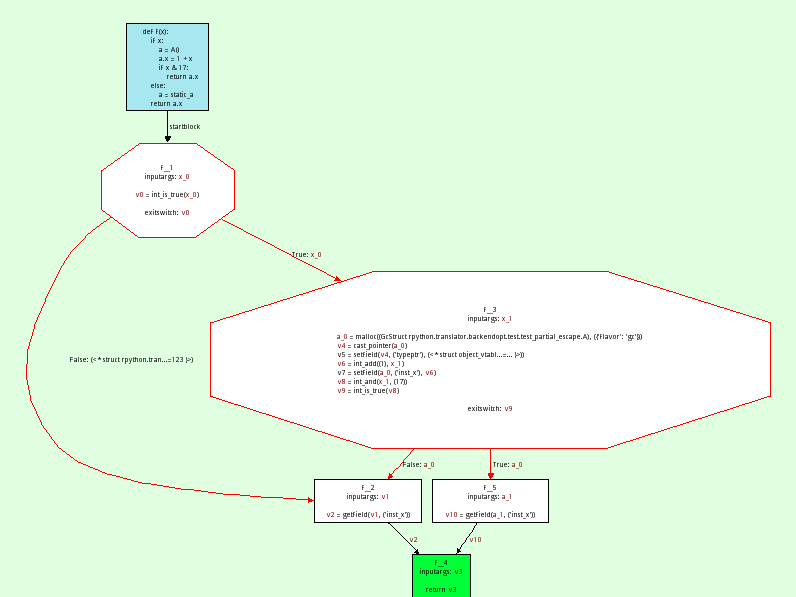
\includegraphics[width=\textwidth]{needs-extra-block-bef.png}
\caption{Extra Block Problem}
\label{figure-8:a}
\end{subfigure}
\begin{subfigure}{0.4\textwidth}
\centering
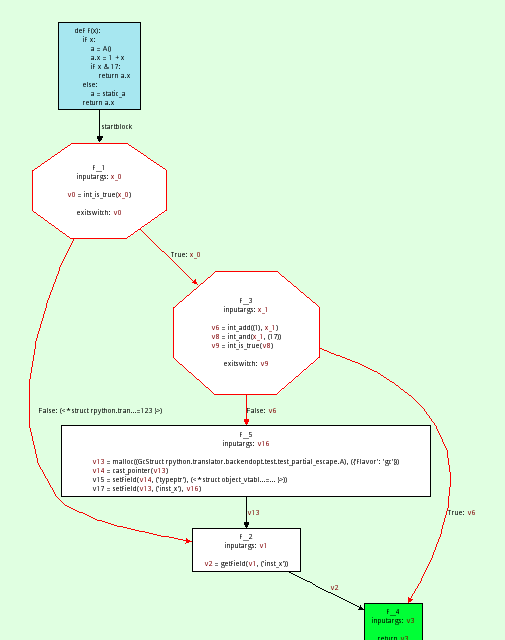
\includegraphics[width=1.05\textwidth]{needs-extra-block-after.png}
\caption{Extra Block Problem Solution}
\label{figure-8:b}
\end{subfigure}
\caption{Screenshot from the diagram editor.} %%%%%%%%%%%%%%%%%%%%%
\end{figure}

Στο \ref{figure-8:b} φαίνεται το διάγραμμα μετά την λύση που εφαρμόσαμε. Το
επιπλέον \texttt{Block} έχει τώρα τον κώδικα δέσμευσης, οπότε αυτό οδηγεί στο
\textit{materialization} του αντικειμένου \textit{μόνο} στο branch που θέλουμε.

Όπως είπαμε η λύση αυτού του θέματος ήταν πολύπλοκη. Η ανεύρεση των περιπτώσεων
που απαιτούνται τα επιπλέον \texttt{Block}s πριν την έναρξη του editing του κάθε
\texttt{Block} ήταν εξαιρετικά πολύπλοκη. Από την άλλη εάν αποφασίζαμε να
αποφανθούμε την ανάγκη των επιπλέον \texttt{Blocks}s κατά το editing, τότε
υπήρχε τεράστιο πρόβλημα στην εισαγωγή του \texttt{Block} καθώς αυτό οδηγούσε
στην ανάγκη επιπλέον ενεργειών για την επεξεργασία των (ήδη-επεξεργασμένων)
\texttt{Link}s και \textit{arguments}. Οπότε αποφασίσαμε στην τοποθέτηση ενός
άδειου \texttt{Block} σε κάθε \texttt{Link} του διαγράμματος! Αυτό φαίνεται στο
διάγραμμα \ref {figure-8c}. Μπορεί με την πρώτη ματιά αυτό να ακούγεται
υπερβολικό και καθόλου αποδοτικό, όμως δεν είναι. Όταν η ειδική
συνάρτηση\footnote{\texttt{(insert\_links())}} – η οποία ανατρέχει το πρόγραμμα
πρώτη πριν την έναρξη της ανάλυσης – ανακαλύψει ένα \texttt{Link} τότε τοποθετεί
ένα άδειο \texttt{Block} στο κέντρο και μεταβάλει αναλόγως τα \textit{in \& out}
\texttt{Link}s του, έτσι ώστε να ``τρέχει" φυσικά στο ενδιάμεσο. Έπειτα η ανάλυση
ξεκινά – τα περισσότερα από αυτά τα καινούργια \texttt{Block}s θα παραμείνουν
άδεια, και στο τέλος θα τρέξει η συνάρτηση \textit{καθαρισμού}
\texttt{eliminate\_empty\_blocks())}, η οποία θα κάνει αυτό ακριβώς που αναφέρει
το όνομά της – θα αφαιρέσει τα άδεια \texttt{Block}s. Επίσης τρέχουμε την
συνάρτηση \texttt{join\_blocks())} η οποία συγχωνεύει τυχών συνεχόμενα
\texttt{Block}s που δεν έχουν λόγο να είναι χωρισμένα (π.χ. \textit{if case}).

\begin{figure}[h]
\centering
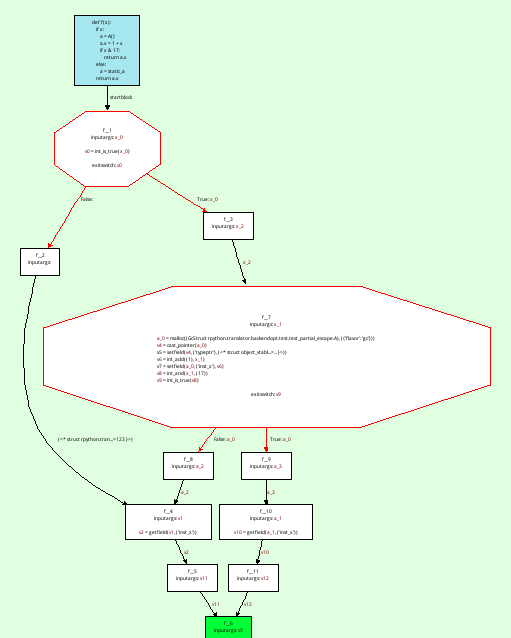
\includegraphics[width=0.8\textwidth]{needs-extra-block-med.png}
\caption{Extra Block Problem Solution (before cleaning up).
Screenshot from the diagram editor.}
\label{figure-8c}
\end{figure}


%------------------------------------------------------------------------------